
\chapter{実験方法}

\section{データセットの作成}
\subsection{撮影環境}
データセットを作成するためにFig.\ref{fig_camera}の環境を構築した.
\begin{figure}[]
  \begin{center}
    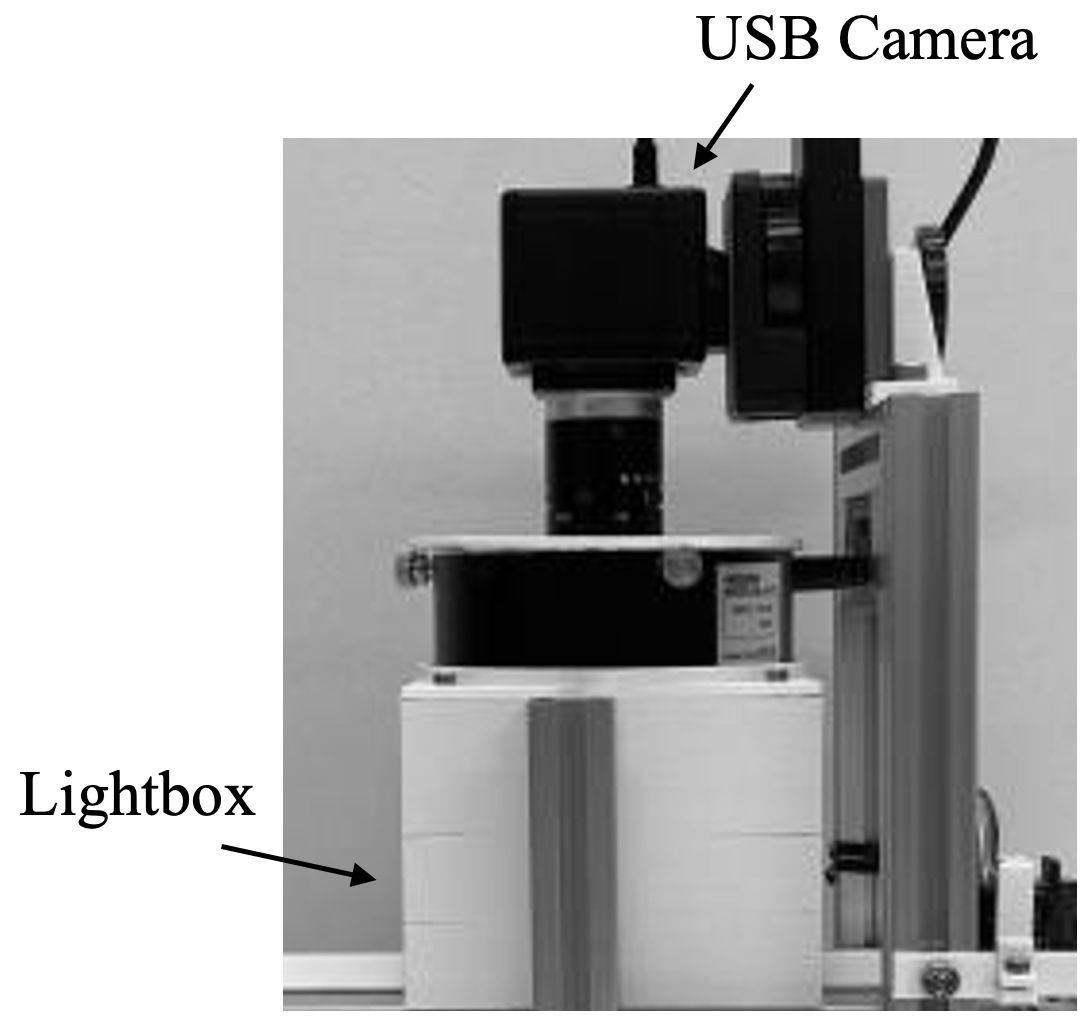
\includegraphics[scale = 0.5]{./chapter3/device.png}
    \caption{撮影環境}
    \label{fig_camera}
  \end{center}
\end{figure}
Webカメラに自作のライトボックスを取り付け,コーヒー豆の撮影時に明度の違いや影を消すための工夫を施した.

\subsection{画像の前処理}
取得画像には以下の前処理を施した.
\begin{enumerate}
\item 画像の2値化
\item 2値化した画像をもちいてコーヒー豆の領域を抽出
\item コーヒー豆の背景を黒でマスキング
\item コーヒー豆の重心を求め,$80\times 80$ピクセルに切り出す
\item コーヒー豆を縦向きに補正
\end{enumerate}
